\section{Passive Sonar}


The sonar subsystem was designed to localize an underwater acoustic beacon emitting at a specific frequency, interpret the tones that it produces and identify the position of the beacon relative to that of the submersible.

\subsection{Principles utilized}

The concept behind passive localization is the detection of "Time
Delays on Arrival" (TDoA) between multiple receivers in a known
geometric configuration. A set of $n$ receivers will produce $n-1$
TDoA values, i.e. one between a reference receiver and every other
receiver in the array.

This concept has limitations: in a 2D (planar) environment, at least
three receivers are required to produce a location. In this case, each
TDoA value, when coupled with the receiver position produces a
hyperbola of possible solutions. To find a point solution, two
TDoA/geometry pairs must be used, and the intersection of the two
resulting hyperbolas calculated. In three dimensions, four receivers
must be used (producing a total of three TDoA values.) This is due to
the fact that each TDoA value/receiver geometry pair produces a
hyperboloid of possible solutions. The intersection of three
hyperboloid surfaces will produce the transmitter location in
question.

Although a closed form solutions exist for both the two and
three-dimensional cases, they are difficult to implement numerically.
To counter this problem, several methods of approximation and
simplification exist: we decided to focus Carter's method\footnote{C. Carter,
  Time Delay Estimation for Passive Signal Processing, IEEE
  Transactions on Acoustics, Speech and Signal Processing, Vol.
  ASSP-29, No.3, 1981, pp. 463-470.}. Carter's method uses the
approximation that the distance between receivers is much smaller than
the distance from receivers to source to approximate the distance and
heading of the beacon in two dimensions. This solution is simple and
holds in a large variety of conditions, making it an ideal candidate
for implementation.


\begin{figure}
  \hrule
  \vspace{.05in}
\centering
\subfigure[Simulated signal perceived by the hydrophones with random noise, echoes and ground references.] {
  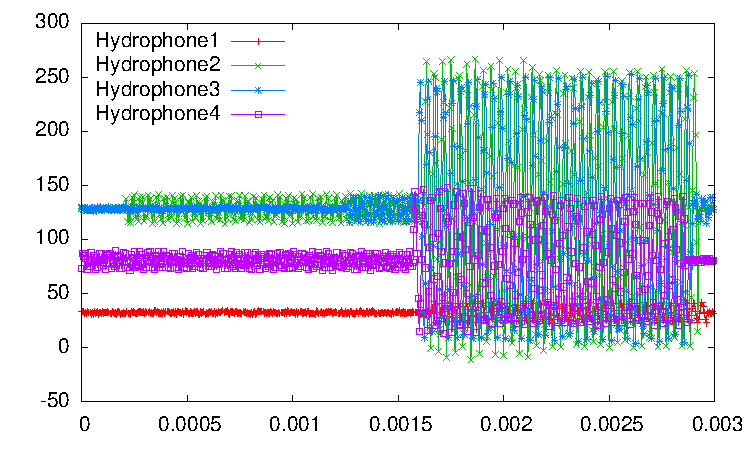
\includegraphics[width=3.3in]{fig/graph}
  \label{fig:bypass_cad}
}
\subfigure[Smoothed and rectified signals before edge detection and correlation.] {
  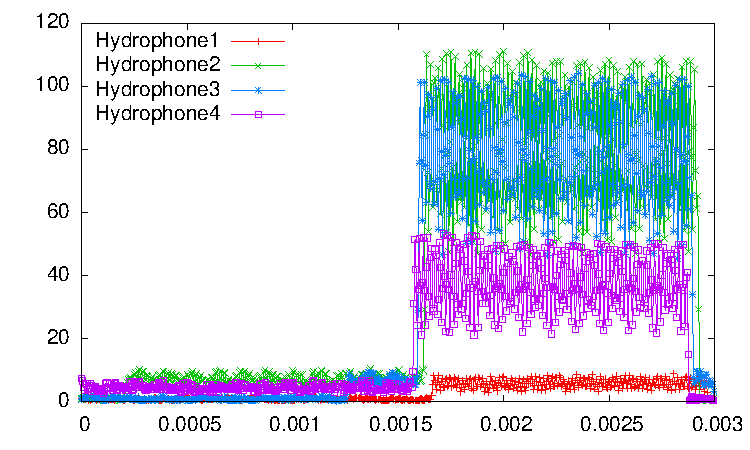
\includegraphics[width=3.3in]{fig/smoothed}
  \label{fig:bypass_eff}
}
  \vspace{.05in}
\hrule
\caption{Examples artificial signals used to experiment with our
  algorithm. The 'x' axis is time and the 'y' axis is amplitude (in
  units matching the intensity of the received signal).}  \label{waves}
\end{figure}


The TDoA method of localization depends very heavily on the accuracy
and precision of the determination of time of arrival of the ping: the time of arrival between the
hydrophones represents a small number of audio samples. This is a
significant challenge when noise and A/D conversion and environment
limitations must be robustly handled. To determine the TDoA of 2
signals, we detect the arriving edge of the ping then improve the
accuracy of our estimation by cross-correlating the two signals (Figure~\ref{waves}).
Cross-correlation  measures the similarity of two
signals. Given two discrete signals $g(n)$ and $h(n)$, the
cross-correlation function $x(d)$ is:

\begin{equation}
x(d) = \sum( g(n)*h(n-d) )
\end{equation}

where $d$ is a phase shift introduced in one of the signals. The
cross-correlation $\sum x(d)$ is then a function of $d$, and is
maximized when the phase-shifted signal $h(n-d)$ matches the signal
$g(n)$ most closely.  To determine the time delay $d$ between signals
from two receivers, the cross-correlation of the two signals is
performed over a range of probable $d$ values.


\subsection{Implementation}
The sonar system was designed to exploit the ample processing power
and familiar debugging environment available  within the main
computer of the AUV. The analog sonar
system consists of two parts: a pre-amplifier with a high
impedance input  followed by
a  filtering and gain stage. The circuit was
specially designed for single supply operation to limit the complexity
of the power supply required.  A dsPIC30F4013 is used to
simultaneously sample and buffer the outputs of the analog stage. The
data is then fed to the main computer using an RS-232 serial interface
for high-level processing and decision making.
